% !TEX root =  main.tex

\section{Empirical Verification and Applications}
\label{sec:empirical}

The convergence rates proven in Section~\ref{sec:convergence} are only
\emph{upper bounds} on the worst case performance we can expect. We will now
examine whether these convergence rates are tight in practice, investigate what happens
when our guidelines are not followed, and outline some possible applications of NMC. 

We start with the following simple model where the exact solution for $I$
can be calculated analytically:
\begin{equation}
\begin{aligned}
\label{eq:model}
& y \sim \mathrm{Uniform}(-1,1), &&
z \sim \mathcal{N}(0,1), \\
& \phi(y,z) = \sqrt{2/\pi}\exp\left(-2(y-z)^2\right), &&
f(y,\gamma(y)) = \log (\gamma (y)) = \log(\E_z[\phi(y,z)]).
\end{aligned}
\end{equation}
Figure~\ref{fig:emprical-conv} shows the corresponding empirical convergence obtained by
applying~\eqref{eq:nested-mc} to~\eqref{eq:model} directly. It shows that, at least in
this case, the theoretical convergence rates from Theorem~\ref{the:Rate} are indeed
realised. The figure also demonstrates the danger of not increasing
$M$ with $N$, showing that the NMC estimator converges to an incorrect solution when $M$
is held constant.  Figure~\ref{fig:tau_sweep} shows the effect of varying $N$ and $M$ for various
fixed sample budgets $T$ and demonstrates that the asymptotically optimal strategy can be suboptimal
for finite budgets.  An extension of this model to a case with multiple levels of nesting is
shown in Appendix~\ref{sec:exp-repeat-app}.

\begin{figure}[t]
	\centering
	\begin{subfigure}[b]{0.49\textwidth}
		\centering
	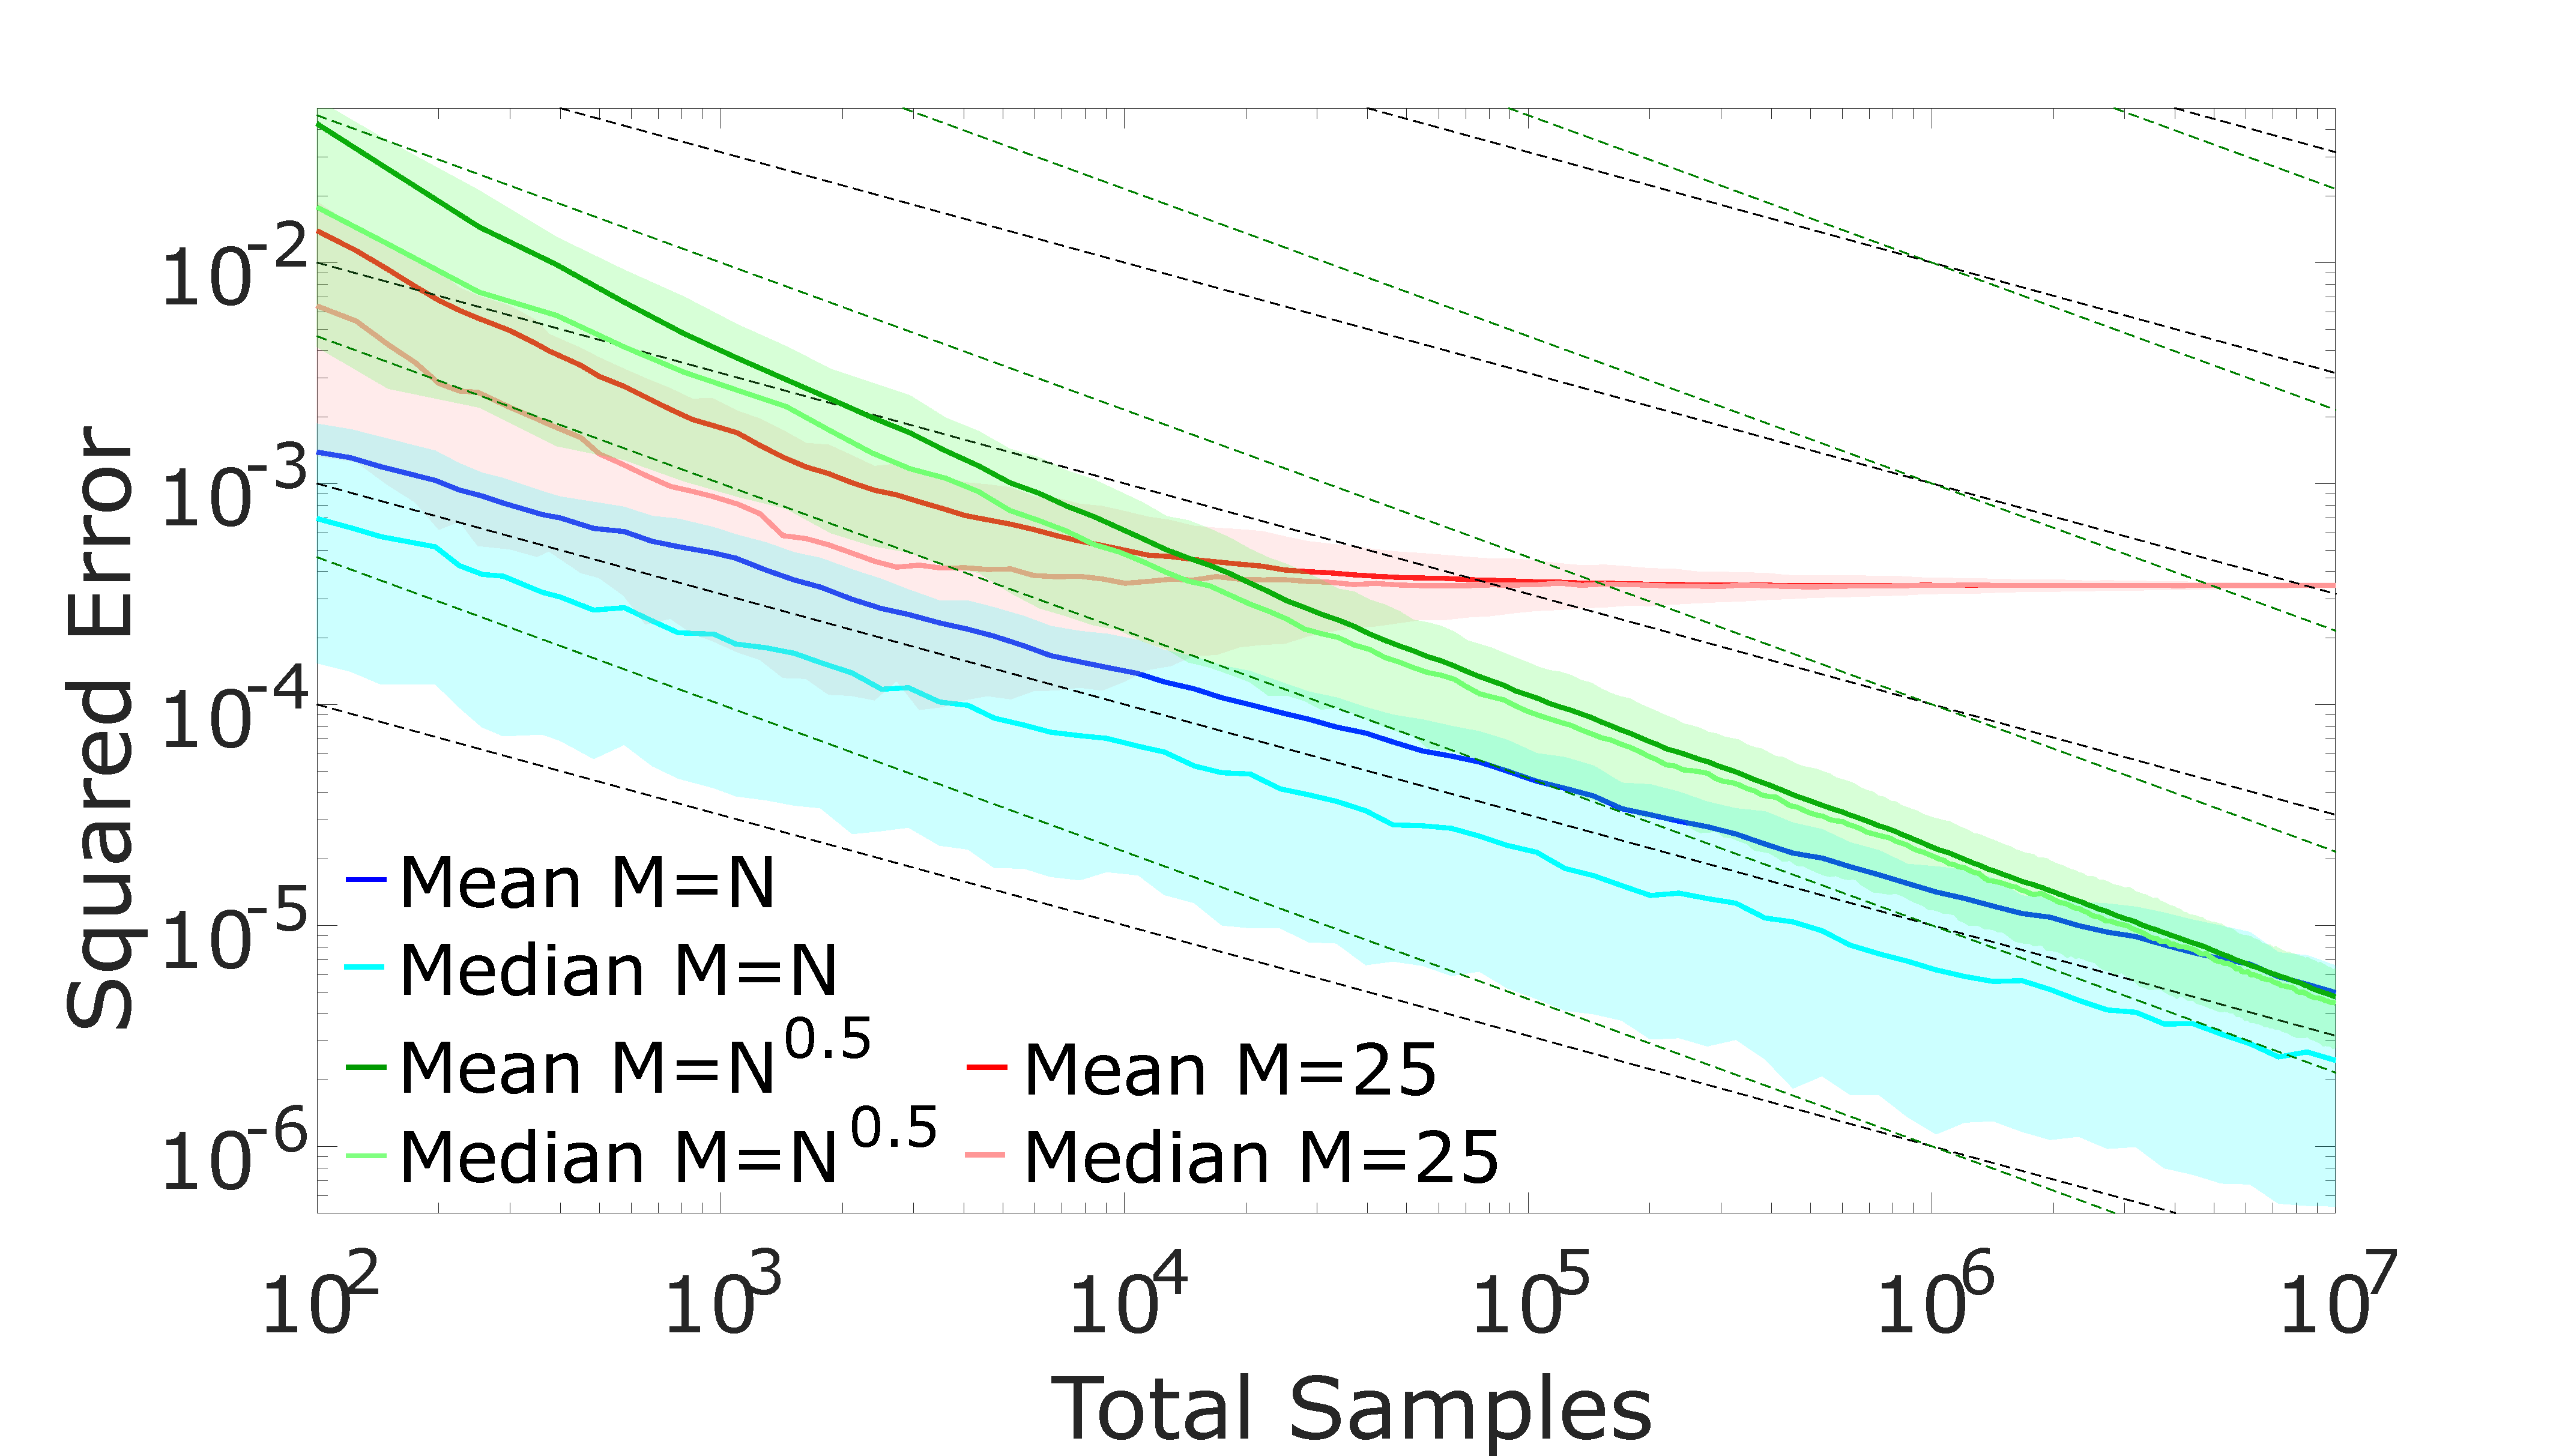
\includegraphics[width=0.99\textwidth,trim={1.5cm 0 3.5cm 0},clip]{gaussian_conv2}
	\caption{Convergence of NMC for different $\tau$. \label{fig:emprical-conv}}
	\end{subfigure}
	\begin{subfigure}[b]{0.49\textwidth}
		\centering
	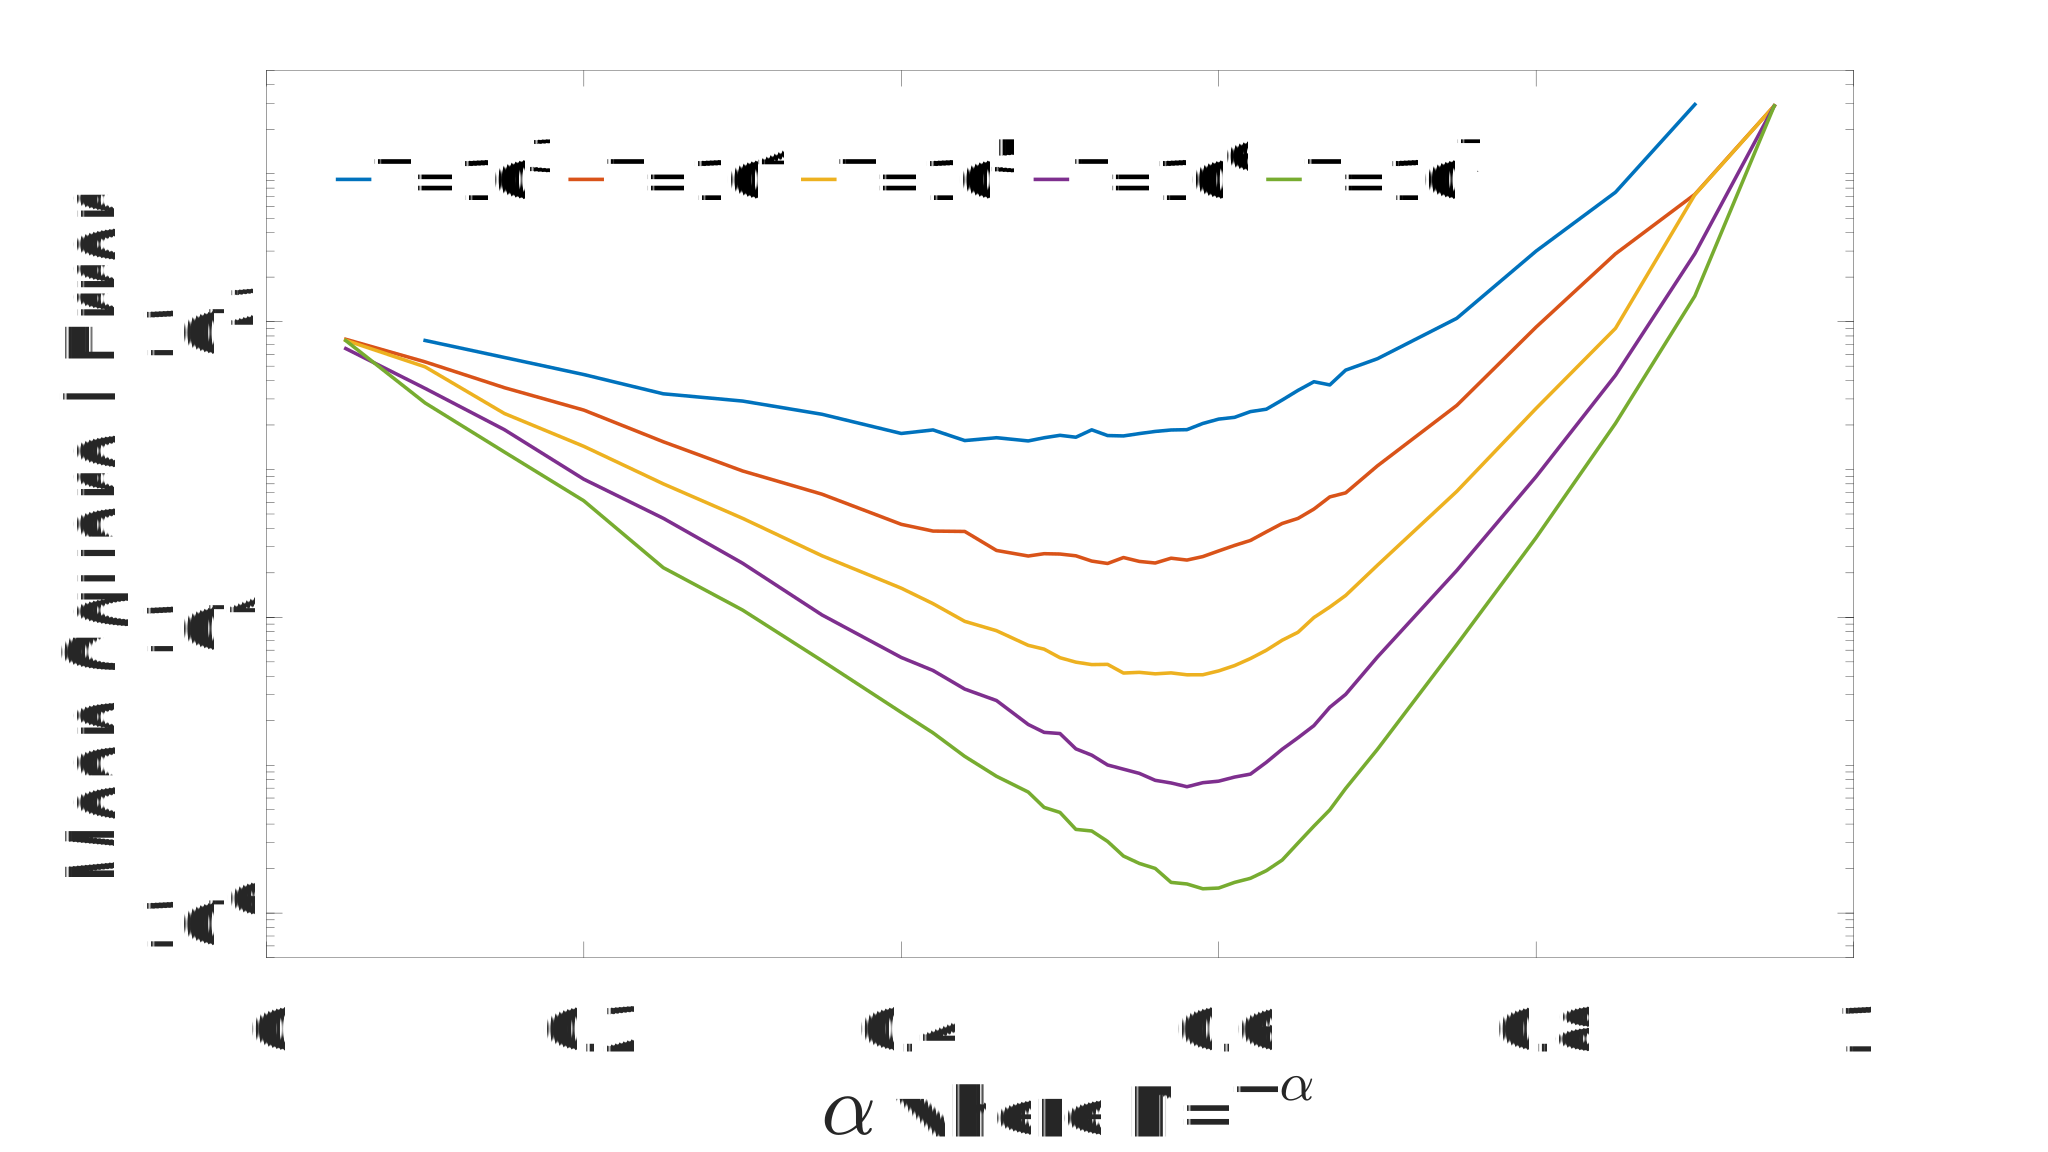
\includegraphics[width=0.99\textwidth,trim={1.5cm 0 3.5cm 0},clip]{tau_sweep}
		\caption{Final error for different $T$ and $N$.\label{fig:tau_sweep}}
	\end{subfigure}
	\caption{Empirical convergence of NMC for~\eqref{eq:model}.  Shown left is the
		convergence in total samples for different ways of setting $M$ and $N$.  
		Results are averaged over 1000 independent runs, while shaded regions give the 25\%-75\% quantiles. We
		see that the theoretical convergence rates (as shown by the dash lines) are observed. 
		The fixed $M$ case converges at the MC error rate, but to a biased solution.
		Shown right is the final error for different total sample budgets
		as a function of $\alpha$ where $N=T^{\alpha}$ and $M=T^{1-\alpha}$ iterations are used for the outer
		and inner estimators respectively.  This shows that even though $\alpha=2/3$ is the
		asymptotically optimal allocation strategy, this is not the optimal solution for
		finite $T$. Nonetheless, as $T$ increases, the optimum value of $\alpha$ increases,
		starting at around $0.5$ for $T=10^3$ and reaching around $0.6$ for $T=10^7$. \vspace{-5pt}}
\end{figure}	

\subsection{Planning Cancer Treatment}
\label{sec:cancer}

We now introduce a real-world example to show the applicability of NMC in a scenario
where the solution is not analytically tractable and conventional MC is insufficient.
Consider a treatment centre assessing a new policy for planning cancer treatments, subject to a budget. 
Clinicians must decide on a patient-by-patient basis whether to administer chemotherapy in the
hope that their tumour will reduce in size sufficiently to be able to perform surgery at a later date.
A treatment is considered to have been successful if the size of the tumour drops below a threshold value in a fixed time window.
The clinicians have at their disposal a simulator for the evolution of tumours with time,
parameterized by both observable values, $y$, such as tumour size, and unobservable values, $z$, such as the patient-specific response to treatment.
Given a set of input parameters, the simulator deterministically returns a binary response $\phi(y,z)\in\left\lbrace 0,1\right\rbrace $, with $\phi(y,z) = 1$ indicating a successful treatment.
To estimate the probability of a successful treatment for a given patient, the clinician must calculate the expected
success over these unobserved variables, namely $\E_{z\sim p(z|y)} [\phi(y,z)]$ where $p(z|y)$ represents a probabilistic
model for the unobserved variables, which could, for example, be constructed based on empirical data.
The clinician then decides whether to go ahead with the treatment for that
patient based on whether the calculated probability of success exceeds a certain threshold $T_{\mathrm{treat}}$.

The treatment centre now wishes to estimate the expected number of patients that will be treated for a given $T_{\mathrm{treat}}$ so that it can minimize this threshold without exceeding its budget.
To do this, it needs to calculate the expectation of the clinician's decisions to administer 
treatment, giving the complete nested expectation for calculating the number of treated patients as
\begin{equation}
	\label{eq:cancer}
I(T_{\mathrm{treat}}) = \E_{y \sim p(y)} \left[\mathbb{I}\left(\E_{z\sim p(z|y)} [\phi(y,z)]>T_{\mathrm{treat}}\right)\right],
\end{equation}
which we propose to estimate using NMC.  Full details on $\phi$, $p(y)$, and $p(z|y)$ are 
provided in Appendix~\ref{sec:cancer_sim_app}.

To verify the convergence rate, we repeat the analysis from Section~\ref{sec:convergence} for the problem defined by~\eqref{eq:cancer} at a fixed value of $T_{\mathrm{treat}}=0.35$. 
The results, shown in Figure~\ref{fig:emperical-conv-cancer}, again verify the theoretical rates. 
By further testing different values of $T_{\mathrm{treat}}$, we found $T_{\mathrm{treat}} \ge 0.125$ (i.e.
go ahead with treatment if the probability of success is 0.125 or greater) to be the optimal under the budget.

\subsection{Bayesian Experimental Design}
\label{sec:bo-design}

In this section we show how our results can be used to derive an improved estimator for the problem of
Bayesian experimental design (BED) in the case where the experiment outputs are discrete.  Due to space
restrictions, this section is necessarily brief, with a full introduction to BED, the derivation of all
the introduced estimators, and additional results provided in Appendix~\ref{sec:exp-design}.

Bayesian experimental design provides a framework for designing experiments in a manner that is optimal from
an information-theoretic viewpoint \citep{chaloner1995bayesian,sebastiani2000maximum}.  Given a prior
$p(\theta)$ on parameters $\theta$ and a corresponding likelihood $p(y|\theta,d)$ for experiment 
outcomes $y$ given a design $d$, the Bayesian optimal design $d^*$ is given by maximizing the mutual
information between $\theta$ and $y$ defined as follows
\begin{align}
\bar{U}(d)=
\int_{\mathcal{Y}}\int_{\Theta} p(y,\theta | d)\log\left(\frac{p(\theta |y, d)}{p(\theta)}\right)d\theta dy. 
\label{eq:u_bar_main}
\end{align}
Finding $d^*$ is challenging as the posterior $p(\theta |y, d)$ is rarely known in closed form.  
However, after appropriate algebraic manipulation, it can be shown that~\eqref{eq:u_bar_main}
is consistently estimated by
\begin{align}
\label{eq:exp-des-nmc-main}
\hat{U}_{\text{NMC}}(d) =
\frac{1}{N} \sum_{n=1}^{N} \left[ \log(p(y_n | \theta_{n,0},d)) 
- \log \left(\frac{1}{M} \sum_{m=1}^{M}p(y_n | \theta_{n,m},d)\right) \right]
\end{align}
where $\theta_{n,m} \sim p(\theta)$ for each $(m,n) \in \{0,\ldots,M\}\times \{1,\ldots,N\}$, 
and $y_n \sim p(y|\theta=\theta_{n,0}, d)$ for each $n \in \{1,\ldots,N\}$.  
This na\"{i}ve NMC estimator has been implicitly used by \cite{myung2013tutorial} and \cite{ouyang2016practical} amongst others and gives a convergence
rate $O(1/M^2+1/N)$ as per Section~\ref{sec:convergence}.

When $y$ can only take on finitely many realisations $y_{1},\dots,y_c$, we use the ideas introduced
in Section~\ref{sec:discrete} to derive the following estimator
\begin{align}
\begin{split}
\label{eq:u_bar_MC_main}
\hat{U}_{R}(d) = &\frac{1}{N} \sum_{n=1}^{N} \sum_{c=1}^{C} p(y_c | \theta_n, d) \log\left(p(y_c | \theta_n, d)\right) \\
&- \sum_{c=1}^{C} \left[\left(\frac{1}{N}\sum_{n=1}^{N} p(y_c | \theta_n, d)\right) \log \left(\frac{1}{N} \sum_{n=1}^{N} p(y_c | \theta_n, d)\right) \right]
\end{split}
\end{align}
where $\theta_n \sim p(\theta)$ for each $n \in \{1,\dots,N\}$.  
As $C$ is a fixed
constant,~\eqref{eq:u_bar_MC_main} converges at the standard MC error rate of $O(1/N)$.  This constitutes
a substantially faster convergence as~\eqref{eq:exp-des-nmc-main} requires a total of $MN$
samples compared to $N$ for~\eqref{eq:u_bar_MC_main}.  To the best of our knowledge, this estimator for this experimental design problem with its superior convergence guarantee has not been introduced in the literature.

We finish by showing that the theoretical advantages of this reformulation also lead to empirical gains in the estimation of $\bar{U}(d)$.  For this we consider a model used in psychology experiments for delay discounting introduced by \cite{vincent2016hierarchical}, details of which are given in Appendix~\ref{sec:exp-design}.  Convergence results
shown in Figure~\ref{fig:exp-conv} demonstrate that the theoretical convergence rates
are observed while results given in Appendix~\ref{sec:exp-design} show that this leads to significant practical gains 
in estimating $\bar{U}(d)$.

\begin{figure}[t]
	\centering
	\begin{subfigure}[b]{0.49\textwidth}
		\centering
				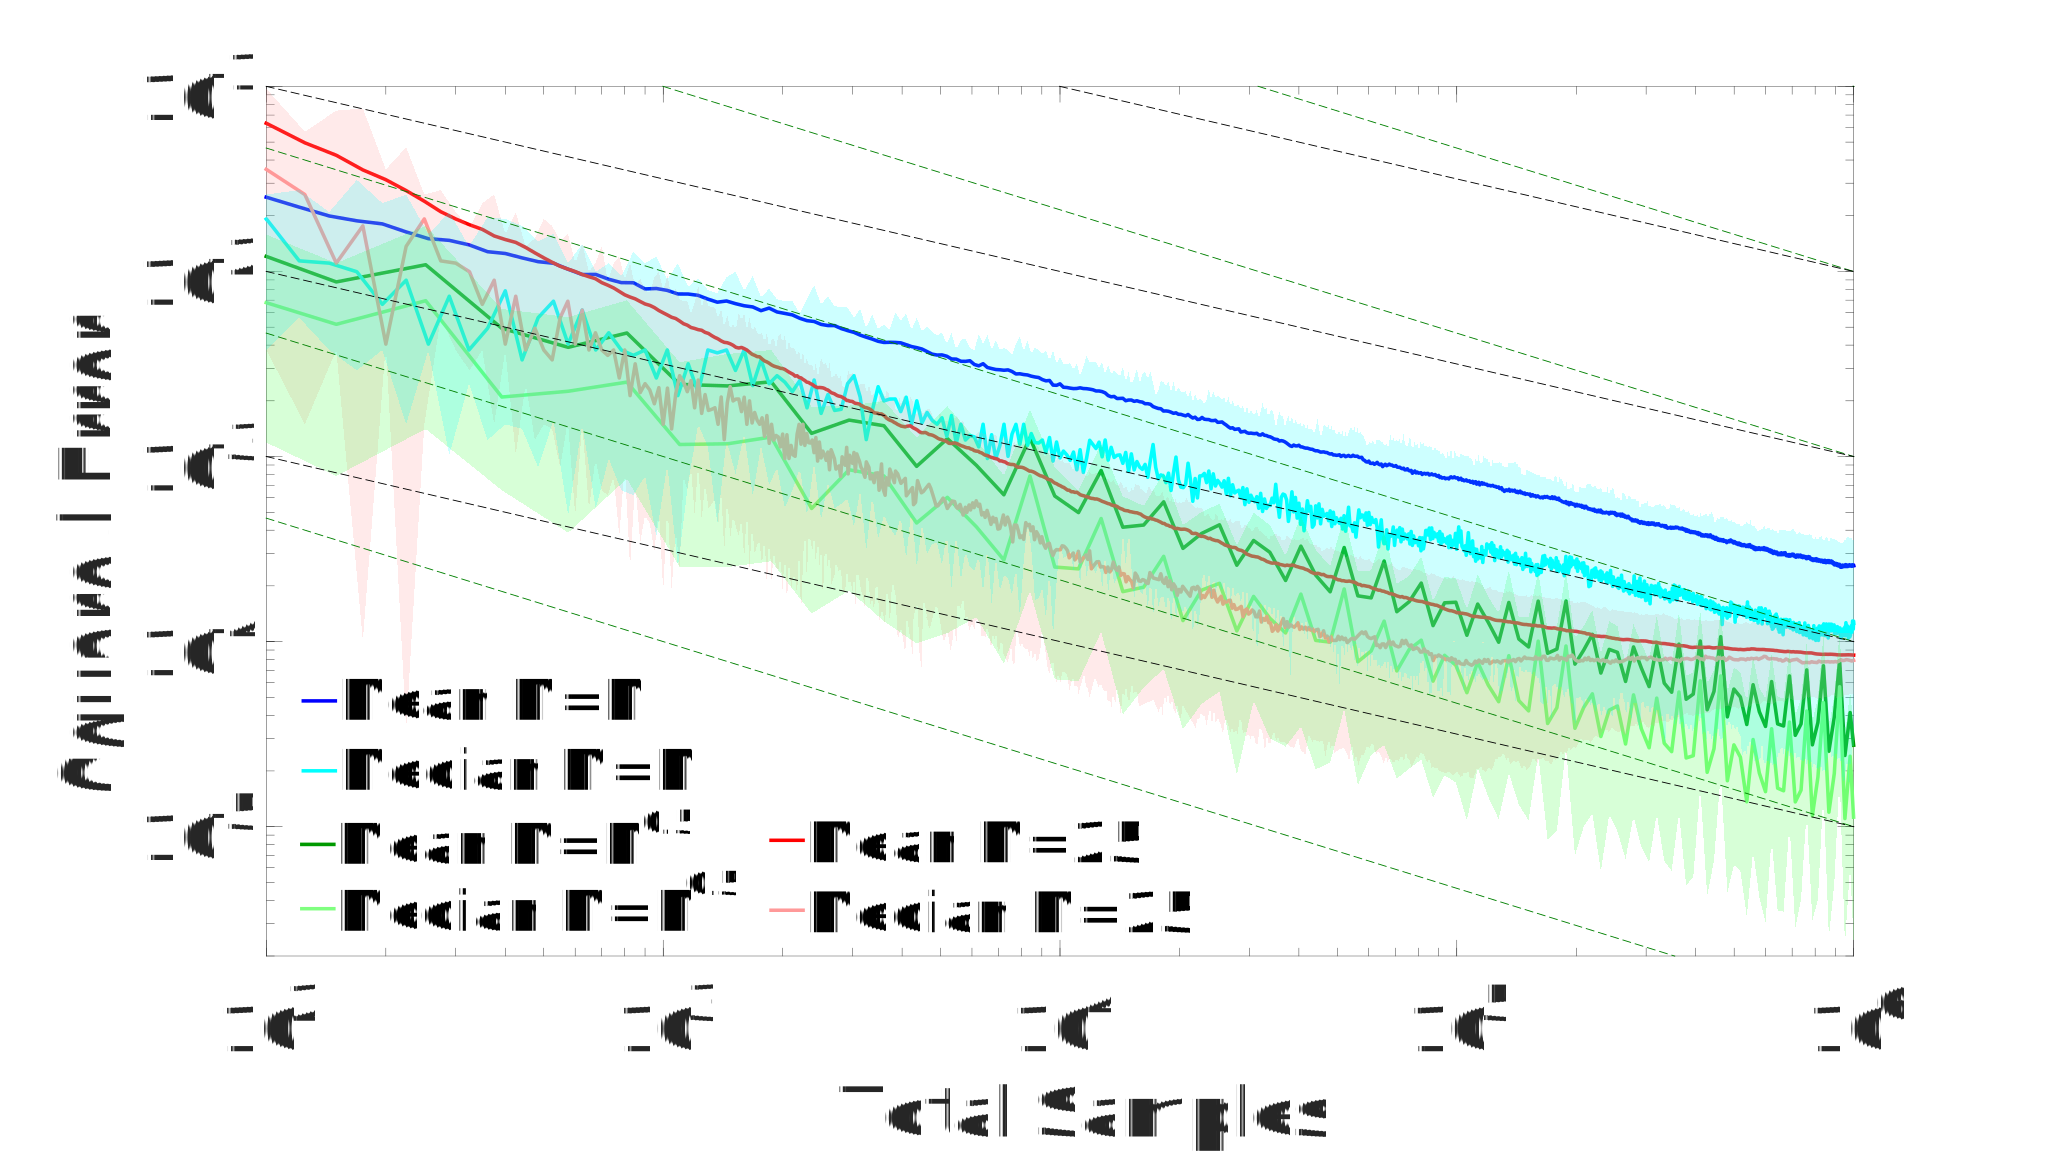
\includegraphics[width=0.99\textwidth,trim={1.5cm 0 3.5cm 0},clip]{canver_conv2}
	\caption{Cancer simulation\label{fig:emperical-conv-cancer}}
	\end{subfigure}
	\begin{subfigure}[b]{0.49\textwidth}
		\centering
			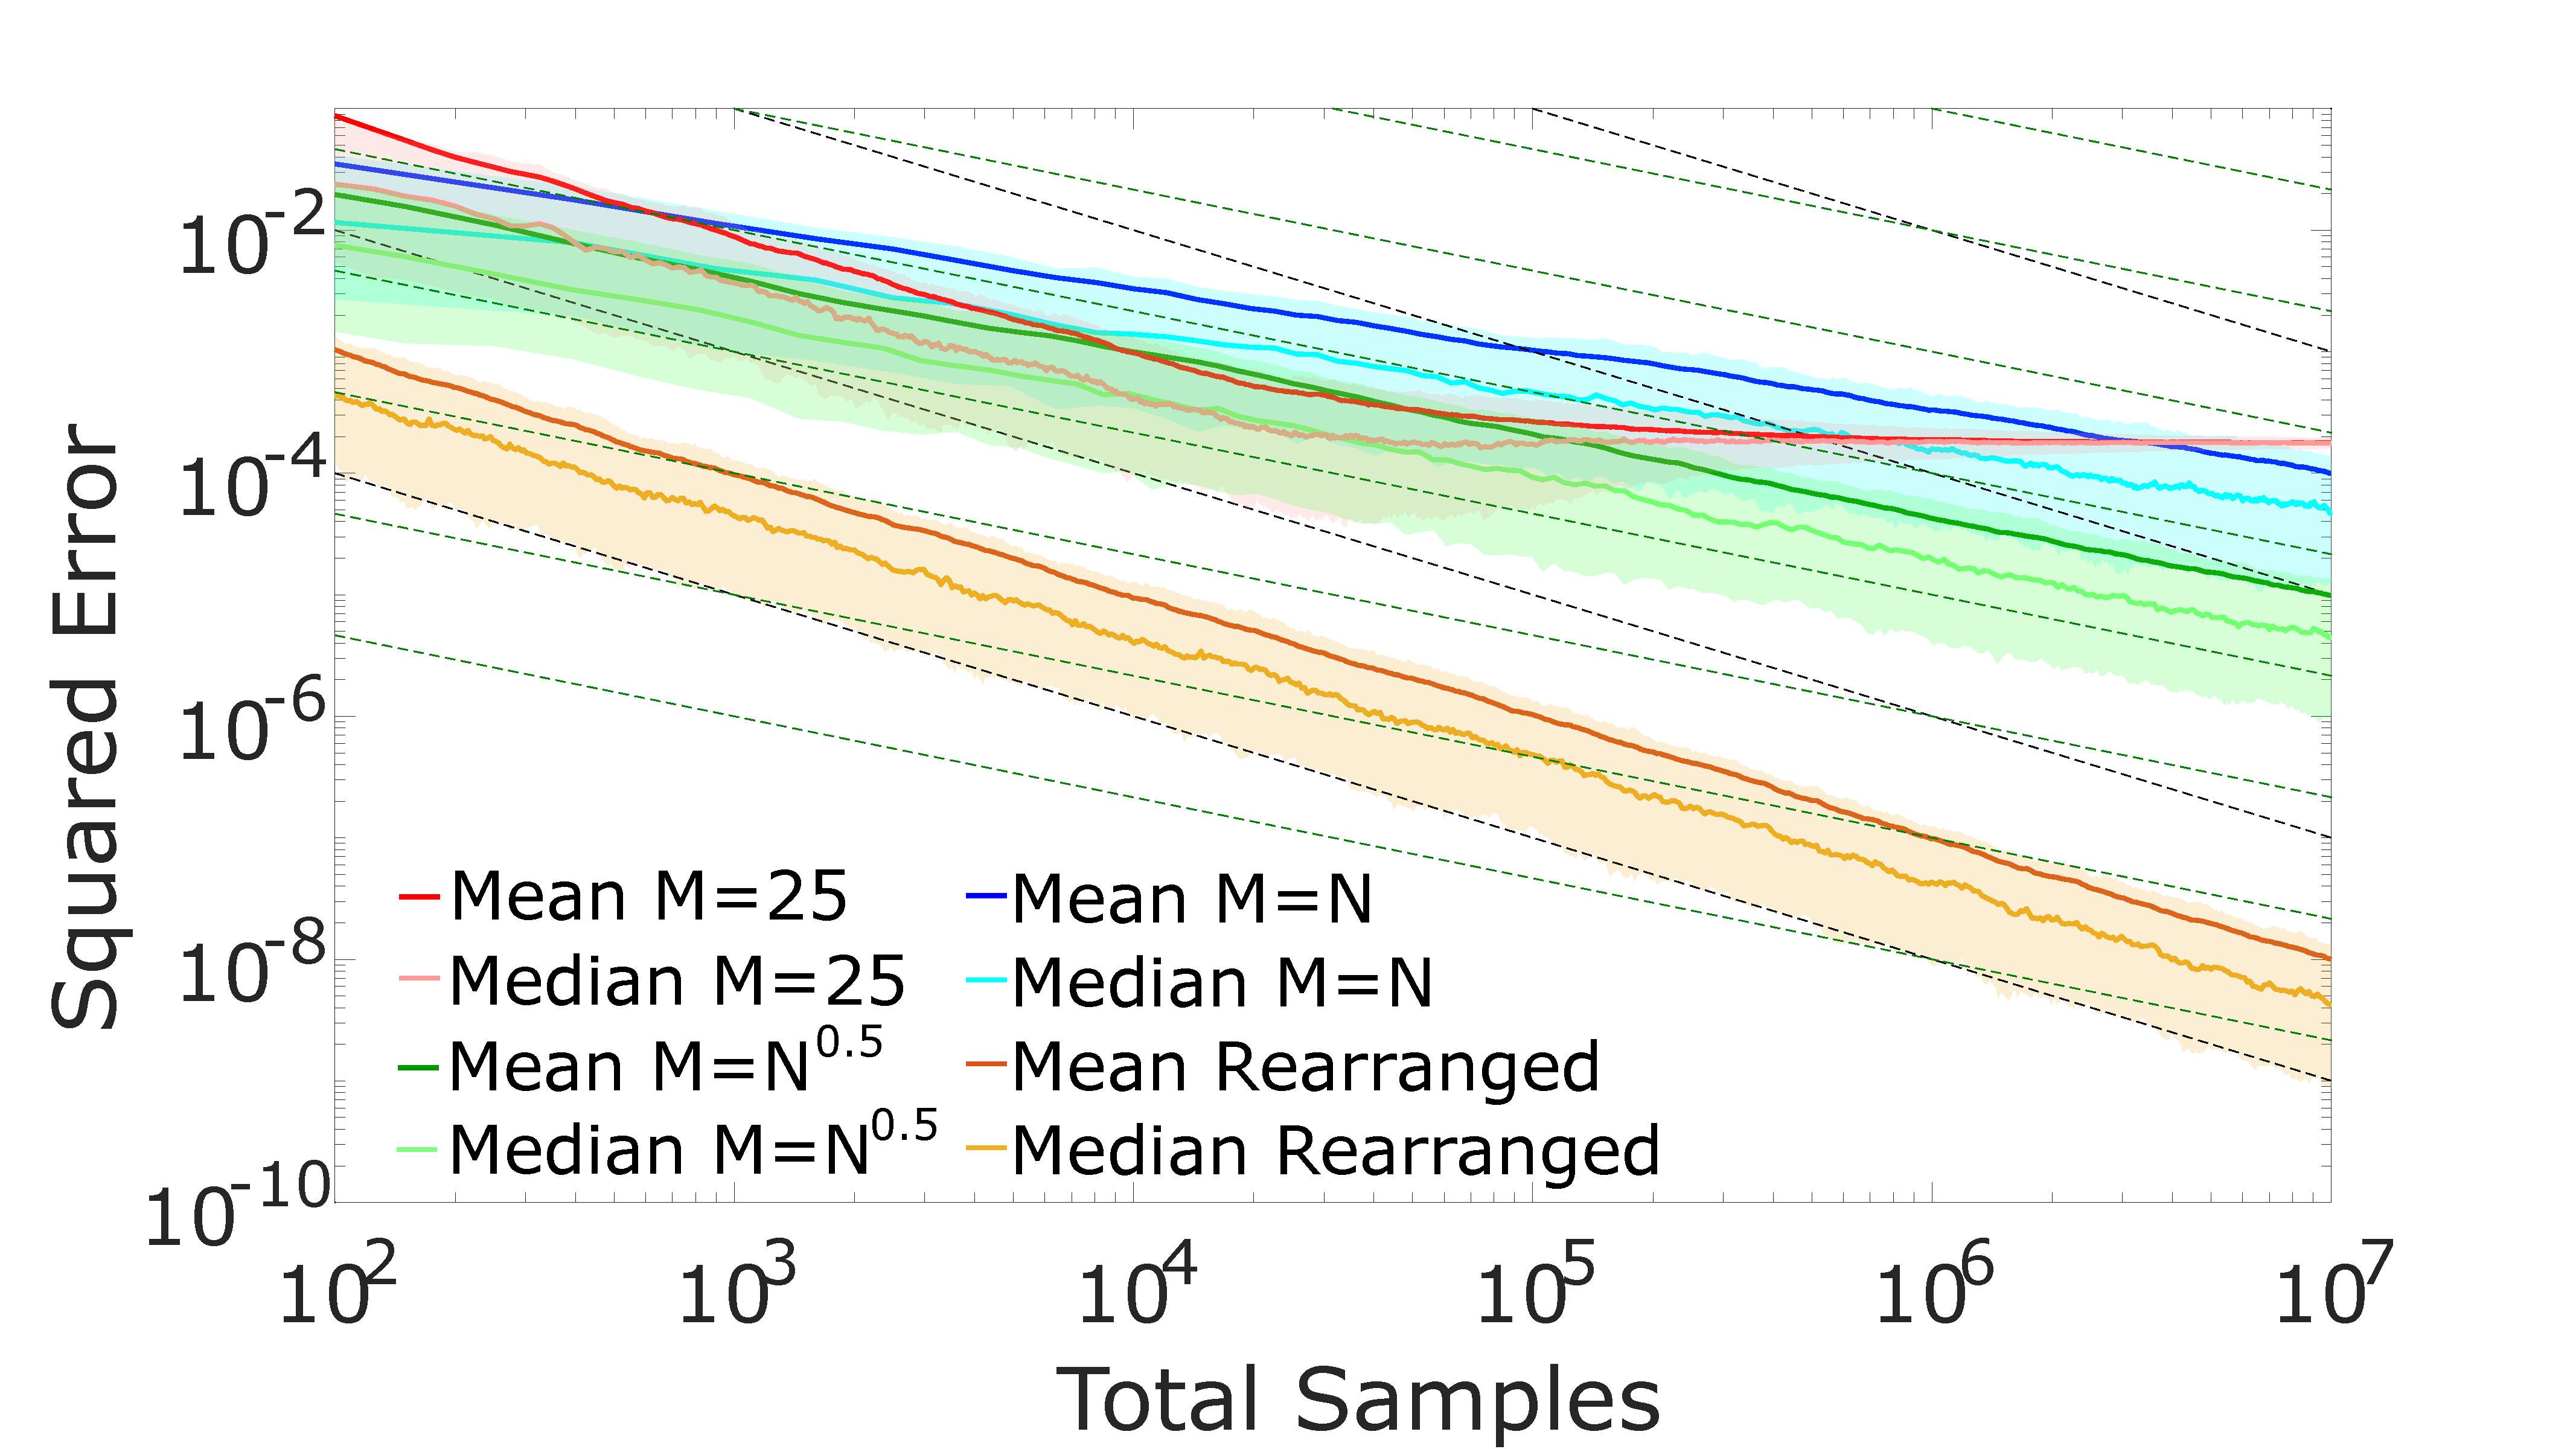
\includegraphics[width=0.99\textwidth,trim={1.5cm 0 3.5cm 0},clip]{exp_conv2}
		\caption{Bayesian experimental design\label{fig:exp-conv}}
	\end{subfigure}
	\caption{Convergence of NMC for cancer simulation and of both NMC and our reformulated
		estimator~\eqref{eq:u_bar_MC_main} for the BED problem.
		A ground truth estimate for the cancer simulation was calculated
		using a single run with $M=10^5$ and $N=10^5$ and using a single run of the reformulated
		estimator with $10^{10}$ for the BED problem.
		Results are averaged over 1000 independent runs, while shaded regions give the 25\%-75\% quantiles. We
		see that the theoretical convergence rates are observed in all cases,
		with the advantages of the reformulated estimator particularly pronounced.
		On the cancer example when $M=\sqrt{N}$ an interesting fluctuation behaviour is observed.  
		Further testing suggests that this originates because the bias of the estimator depends in
		a fluctuating manner on the value of $M$ as the binary output of $\phi(y,z)$ creates a quantization
		effect on the possible estimates for $\hat{\gamma}$.  This effect is also observed for the $M=N$ case,
		but is less pronounced. \vspace{-5pt}}
\end{figure}
